\documentclass{beamer}
\usepackage[ngerman]{babel}
\usepackage[T1]{fontenc}	
\usepackage[utf8]{inputenc}
\usepackage{hyperref}
\usepackage[]{animate}
\usepackage{color}
\usepackage{xcolor}

\newcommand{\ra}{$\rightarrow~$}
\newcommand{\Ra}{$\Rightarrow~$}
\newcommand{\Rra}{$\Rrightarrow~$}

%........................
\usetheme{Frankfurt}
\usecolortheme{dolphin}
%........................
\begin{document}
	\title[]{Das verrückte Labyrinth}	
	\subtitle{Assignment02}
	\author{Daniel Deuscher, Marvin Röck, Rehan App\\ (Team02)}
	\institute{Eberhard Karls Universität Tübingen\\Programmierprojekt Sommersemester 2016}
	\date{\today}
	 
	\begin{frame}
		\maketitle
	\end{frame}
	 
	\section{Bedienungsoberfläche(GUI)}
		%+++++++++++++++++++++++++++++++++++++++++++++++++++++++
		%FRAME 1:
	    \label{Frame1}	
		\begin{frame}
			\frametitle{Bedienungsoberfläche(GUI)}
			\begin{block}{menu}
				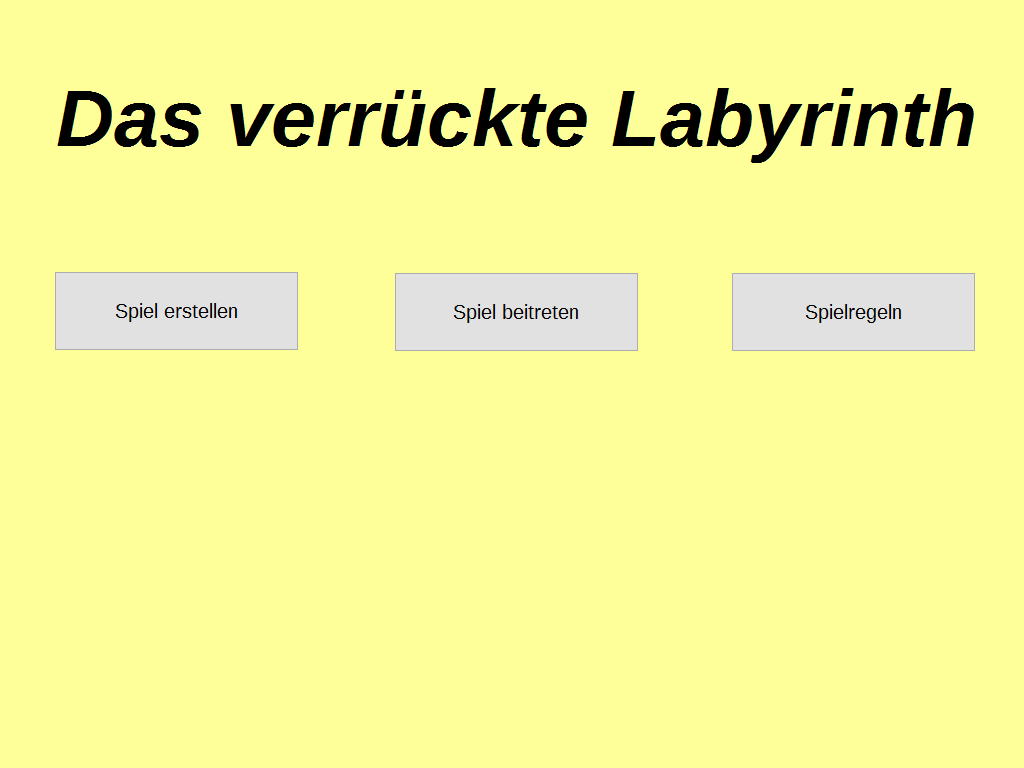
\includegraphics[width = 10.8cm, height = 6cm]{BilderGUI/01-titelpage.png}
			\end{block}		
		\end{frame}
		%========================================================

		%+++++++++++++++++++++++++++++++++++++++++++++++++++++++
		%FRAME 2:
	    \label{Frame2}	
		\begin{frame}
			\frametitle{Bedienungsoberfläche(GUI)}
			\begin{block}{Game rules}
				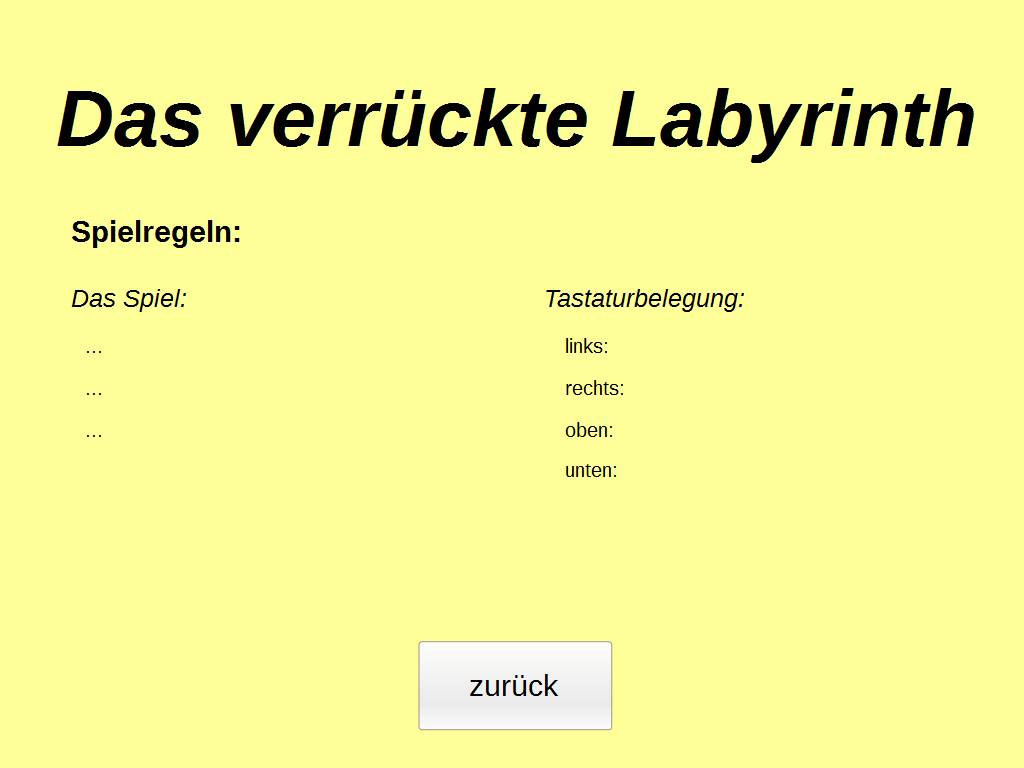
\includegraphics[width = 10.8cm, height = 6cm]{BilderGUI/02-spielregeln.png}
			\end{block}		
		\end{frame}
		%========================================================

		%+++++++++++++++++++++++++++++++++++++++++++++++++++++++
		%FRAME 3:
	    \label{Frame3}	
		\begin{frame}
			\frametitle{Bedienungsoberfläche(GUI)}
			\begin{block}{set Game}
				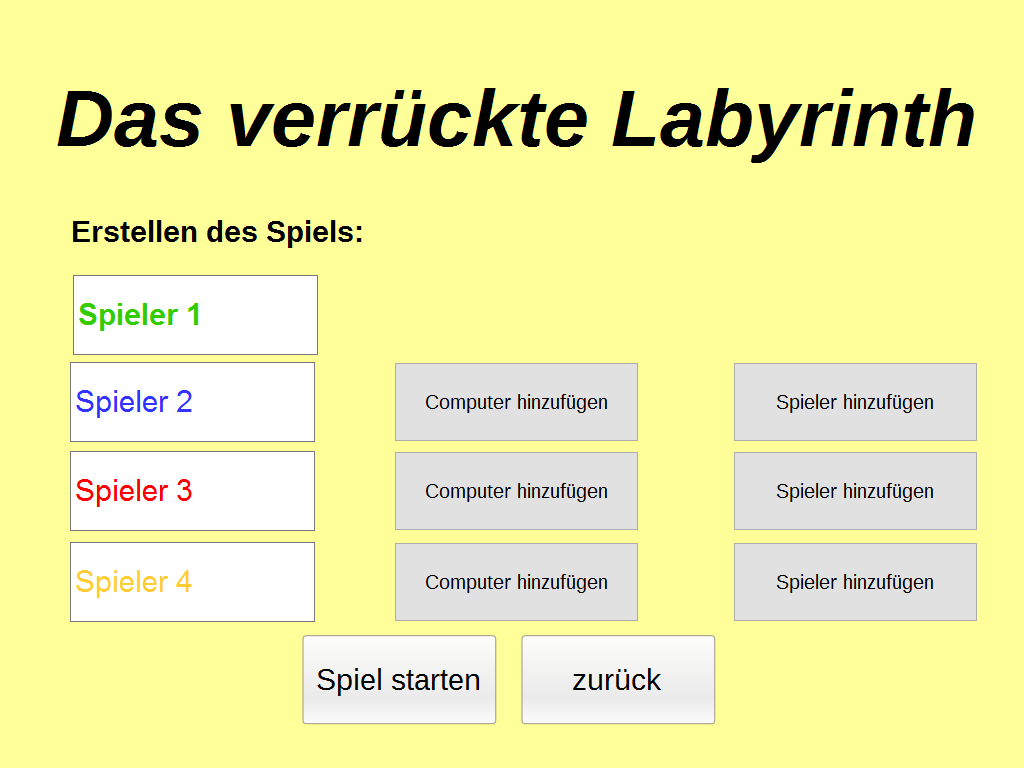
\includegraphics[width = 10.8cm, height = 6cm]{BilderGUI/03-titelhost.png}
			\end{block}		
		\end{frame}
		%========================================================


		%+++++++++++++++++++++++++++++++++++++++++++++++++++++++
		%FRAME 4:
	    \label{Frame4}	
		\begin{frame}
			\frametitle{Bedienungsoberfläche(GUI)}
			\begin{block}{host new game}
				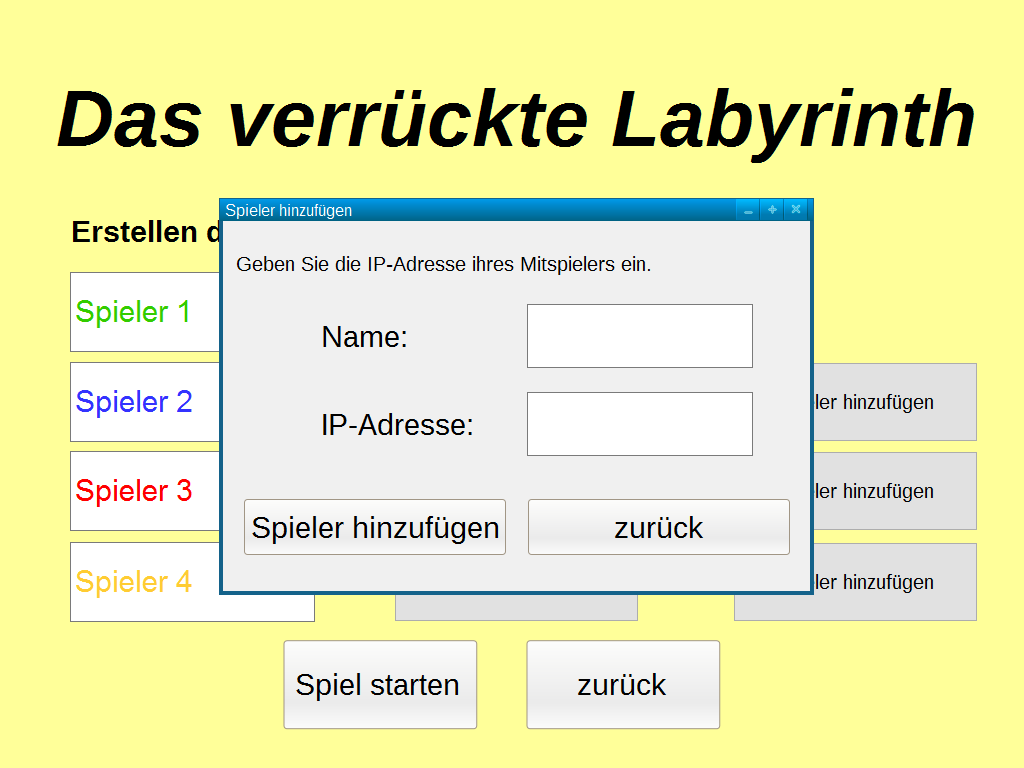
\includegraphics[width = 10.8cm, height = 6cm]{BilderGUI/04-titelhostnewplayer.png}
			\end{block}		
		\end{frame}
		%=======================================================


		%+++++++++++++++++++++++++++++++++++++++++++++++++++++++
		%FRAME 5:
	    \label{Frame5}	
		\begin{frame}
			\frametitle{Bedienungsoberfläche(GUI)}
			\begin{block}{join Game online}
				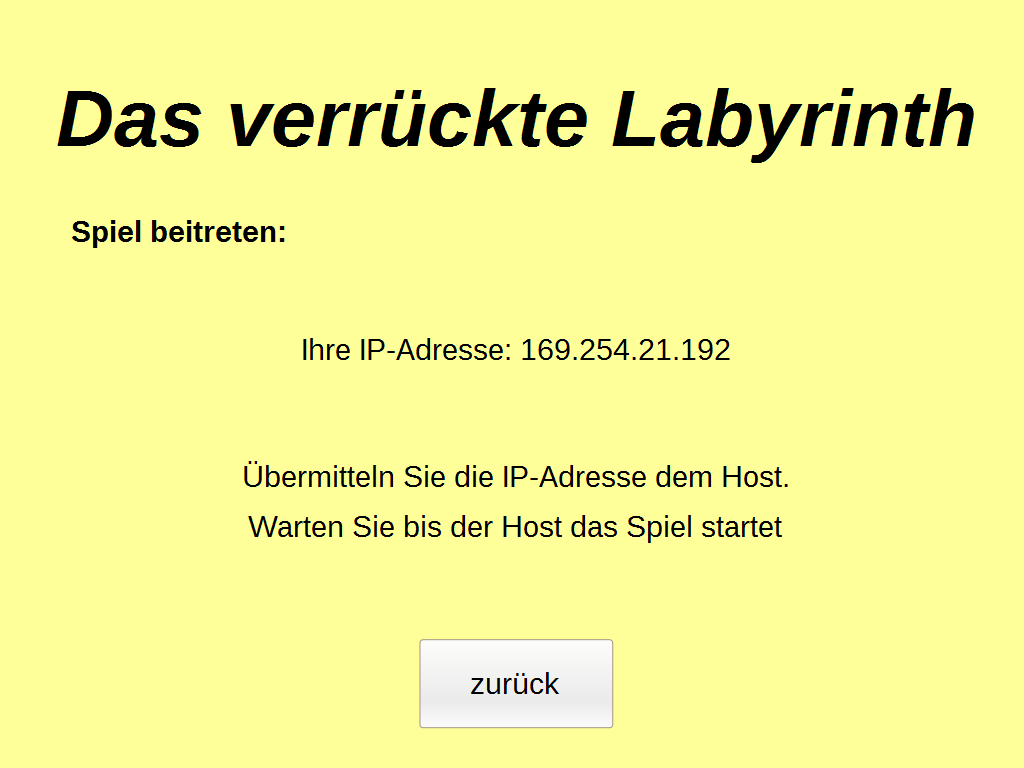
\includegraphics[width = 10.8cm, height = 6cm]{BilderGUI/05-titeljoin.png}
			\end{block}		
		\end{frame}
		%=======================================================


		%+++++++++++++++++++++++++++++++++++++++++++++++++++++++
		%FRAME 6:
	    \label{Frame6}	
		\begin{frame}
			\frametitle{Bedienungsoberfläche(GUI)}
			\begin{block}{game}
				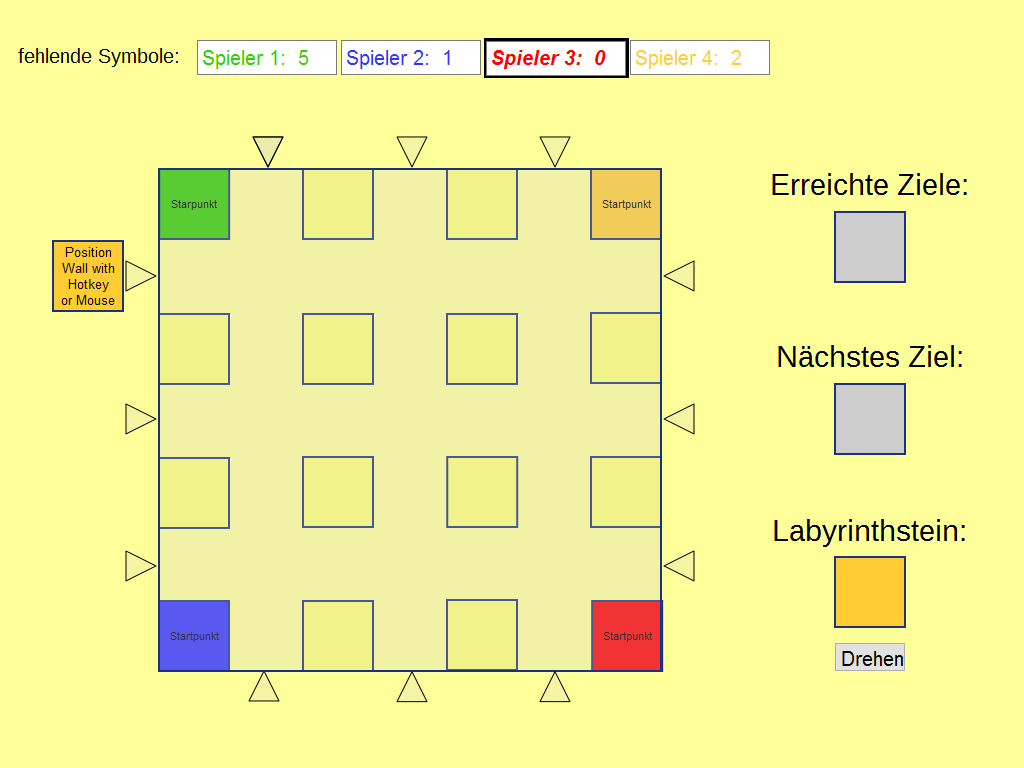
\includegraphics[width = 10.8cm, height = 6cm]{BilderGUI/06-game.png}
			\end{block}		
		\end{frame}
		%=======================================================

		%+++++++++++++++++++++++++++++++++++++++++++++++++++++++
		%FRAME 7:
	    \label{Frame7}	
		\begin{frame}
			\frametitle{Bedienungsoberfläche(GUI)}
			\begin{block}{game end}
				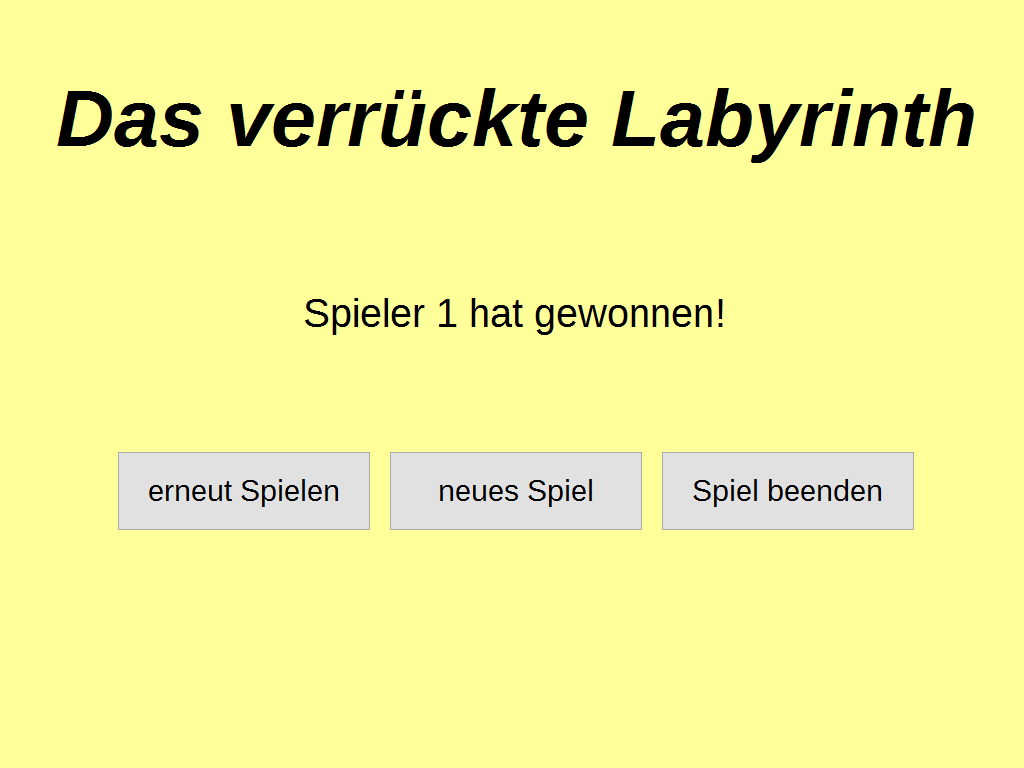
\includegraphics[width = 10.8cm, height = 6cm]{BilderGUI/07-end.png}
			\end{block}		
		\end{frame}
		%======================================================				
		
		\section{Spiel-Engine}
		%+++++++++++++++++++++++++++++++++++++++++++++++++++++++
		%FRAME 7:
	    \label{Frame7}	
		\begin{frame}
			\frametitle{Spiel-Engine}
			\begin{block}{Klassendiagram}
				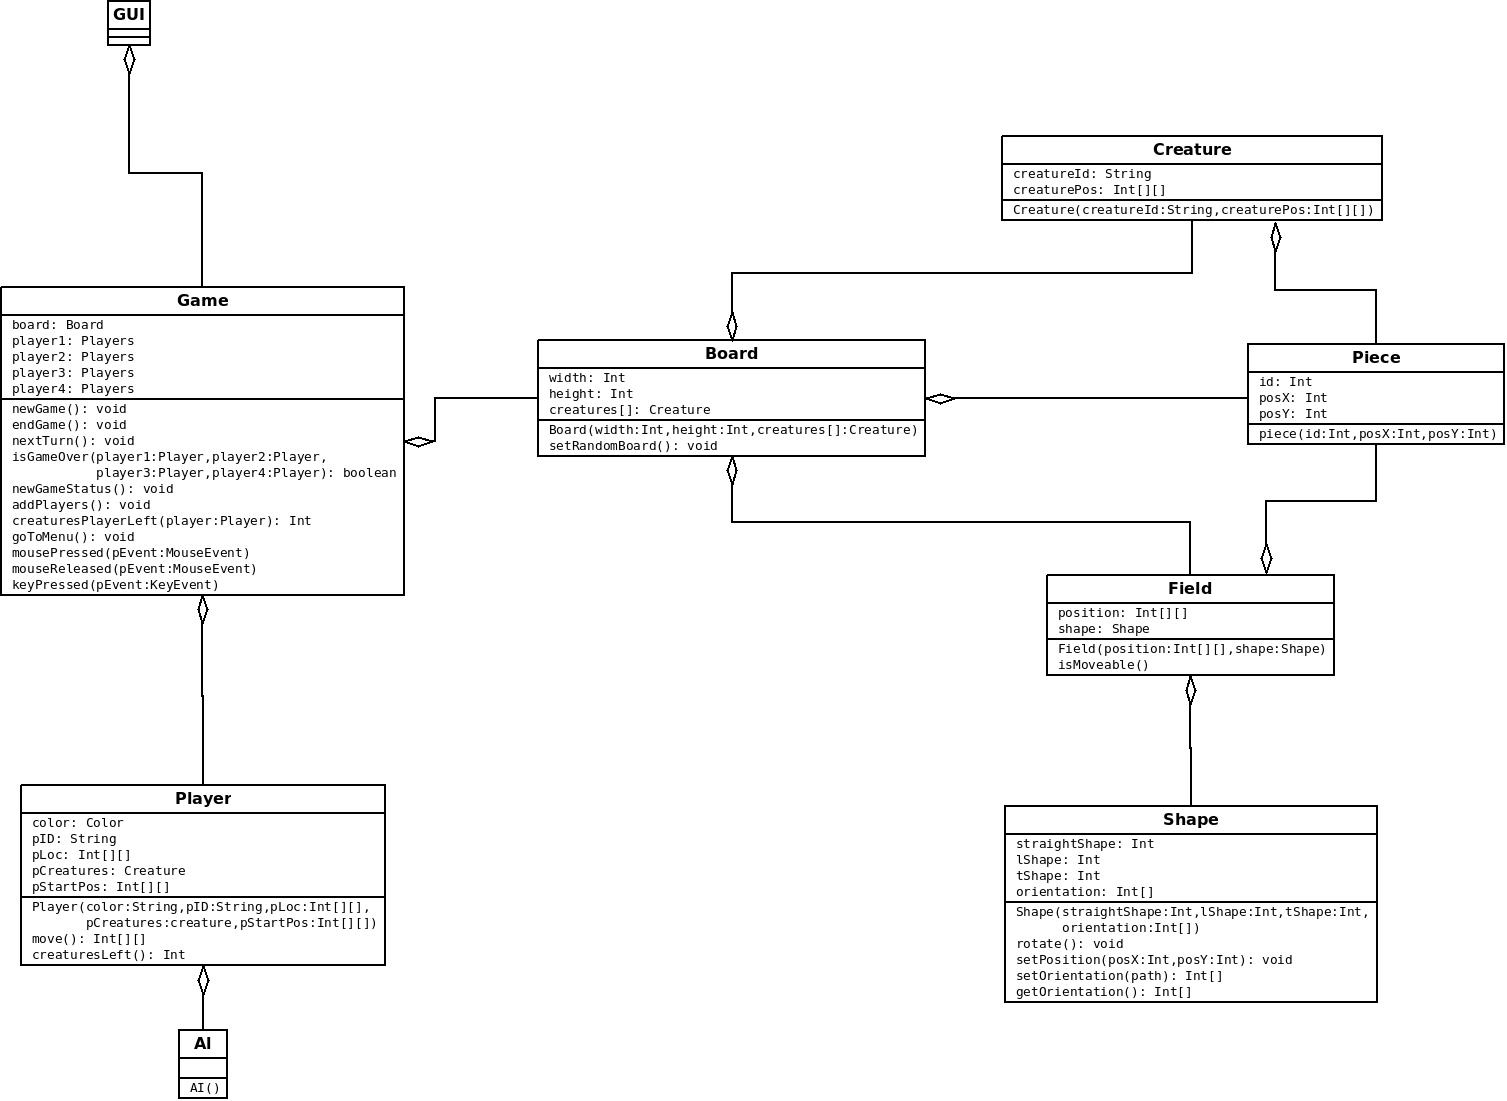
\includegraphics[width = 10.8cm, height = 6cm]{UML/umltest.jpeg}
			\end{block}		
		\end{frame}
		%======================================================												
\end{document}